% Copyright (c) 2009-2015 Ilya Palachev <iliyapalachev@gmail.com>

\documentclass[a4paper, 10pt]{article}
\usepackage[pass,paperwidth=17cm,paperheight=24cm]{geometry}


\usepackage[utf8]{inputenc}
\usepackage[english,russian]{babel}
\usepackage{graphicx}
\usepackage{wrapfig}
\usepackage{amsmath,amssymb}

% Package that enables usage of theorems and definition designed in a 
% standard way.
% http://en.wikibooks.org/wiki/LaTeX/Theorems
\usepackage{amsthm}

% Create environment for smart definitions
\theoremstyle{definition}
\newtheorem{SmartDefinition}{Определение}

% Create environment for smart theorems
\theoremstyle{plain}
\newtheorem{SmartTheorem}{Теорема}

% Create environment for smart lemmas
\theoremstyle{plain}
\newtheorem{SmartLemma}{Лемма}

\title{МЕТОД ВЫЯВЛЕНИЯ ИЗБЫТОЧНЫХ УСЛОВИЙ В ЗАДАЧЕ ВОССТАНОВЛЕНИЯ ТЕЛ ПО ОПОРНЫМ
ФУНКЦИЯМ И ЕГО ПРИЛОЖЕНИЕ К ЗАДАЧЕ ВОССТАНОВЛЕНИЯ ТЕЛ ПО ТЕНЕВЫМ КОНТУРАМ}
\author{Палачев\,И.\,А.}

\begin{document}
\maketitle
\begin{abstract}
 Производится обзор методов восстановления геометрических тел (двумерных и
 трехмерных) по измерениям опорной функции. Рассматривается задача линейного
 программирования, лежащая в основе одного из этих методов. Доказывается
 достаточное условие избыточности ограничений задачи, позволяющее значительно
 уменьшить число ограничений. Рассматривается интерпретация теневых контуров
 как набора измерений опорной функции. Приводятся результаты проверки
 алгоритма на реальных данных, полученных из производственных теневых контуров.
\end{abstract}

\textbf{Ключевые слова:} опорная функция, восстановление геометрических тел,
линейное программирование, квадратичное программирование, теневой контур,
преобразование двойственности

\textbf{1. Введение.} Поводом для данного исследования послужила задача
восстановления трехмерных тел по теневым контурам, которая возникает при
построении моделей драгоценных камней в ювелирной промышленности. Теневые
контуры получаются с помощью фотографирования камня, стоящего на вращающейся
подставке. В результате обработки растрового изображения (фотографии) получается
теневой контур --- многоугольник, являющийся границей тени камня на некоторой
вертикальной плоскости.

При изучении данного вопроса было замечено его удивительное сходство с другими
задачами, имевшими совершенно иное прикладное происхождение и, как оказалось,
изучавшимися в иностранной научной литературе в течение последних почти 30 лет.
Ниже будет приведен краткий обзор этих задач и методов их решения.

Статья преследует двоякую цель. Во-первых, показать что методы
восстановления геометрических тел по измерениям опорной функции применимы к
исходной прикладной задаче, т. е. что теневые контуры можно интерпретировать
как набор измерений опорной функции тела. Во-вторых, доказать свойство
одного из методов, позволяющее значительно ускорить алгоритм решения задачи.

\textbf{2. Основные определения.} Как известно (см. например,
\cite{Ghosh:1998:SFR:307150.307167}), всякое выпуклое тело в $\mathbb{R}^{n}$
однозначно определяется своей опорной функцией:

\begin{SmartDefinition}
 \label{def:support-function}
 \textbf{Опорной функцией} выпуклого тела $K \subset \mathbb{R}^{n}$
 называется
 $h_{K}: \mathbb{R}^{n} \to \mathbb{R}_{+}$:

 \begin{equation}h_{K}(u) = \sup \limits_{x \in K}(x, u)\end{equation}
\end{SmartDefinition}

Поскольку опорная функция является мультипликативной, её часто определяют только
на единичной сфере $S^{n - 1} \subset \mathbb{R}^{n}$. Если тело $K$ содержит
начало координат $O$ в своей внутренности, то его опорная функция положительна.

Допустим, что имеется некоторое реальное физическое тело $K$, для которого
получены приближенные значения $h_{1}, h_{2}, \ldots, h_{m}$ опорной функции
$h_{K}$ на \textit{конечном наборе} единичных векторов
$u_{1}, u_{2}, \ldots, u_{m}$:

\begin{equation}
 h_{i} = h_{K}(u_{i}) + \varepsilon_{i}, \;\; i = 1, 2, \ldots, m,
\end{equation}

где $\varepsilon_{i}$ --- погрешность измерения величины $h_{i}$. Для краткости
здесь и далее будем называть векторы $u_{i}$ \textit{опорными направлениями},
$h_{i}$ --- \textit{опорными числами}, а плоскости, задаваемые уравнениями
$(x, u_{i}) = h_{i}$, --- \textit{опорными плоскостями}.

\begin{SmartDefinition}
 \label{def:consistency}
 Опорные числа $h_{1}, h_{2}, \ldots, h_{m}$ по направлениям \\
 $u_{1}, u_{2}, \ldots, u_{m}$ называются \textbf{согласованными}, если
 существует такое выпуклое тело  $K^{*} \subset \mathbb{R}^{n}$, что
 $h_{K^{*}}(u_{i}) = h_{i}$
\end{SmartDefinition}

\begin{wrapfigure}{r}{0.5\textwidth}
 \begin{center}
  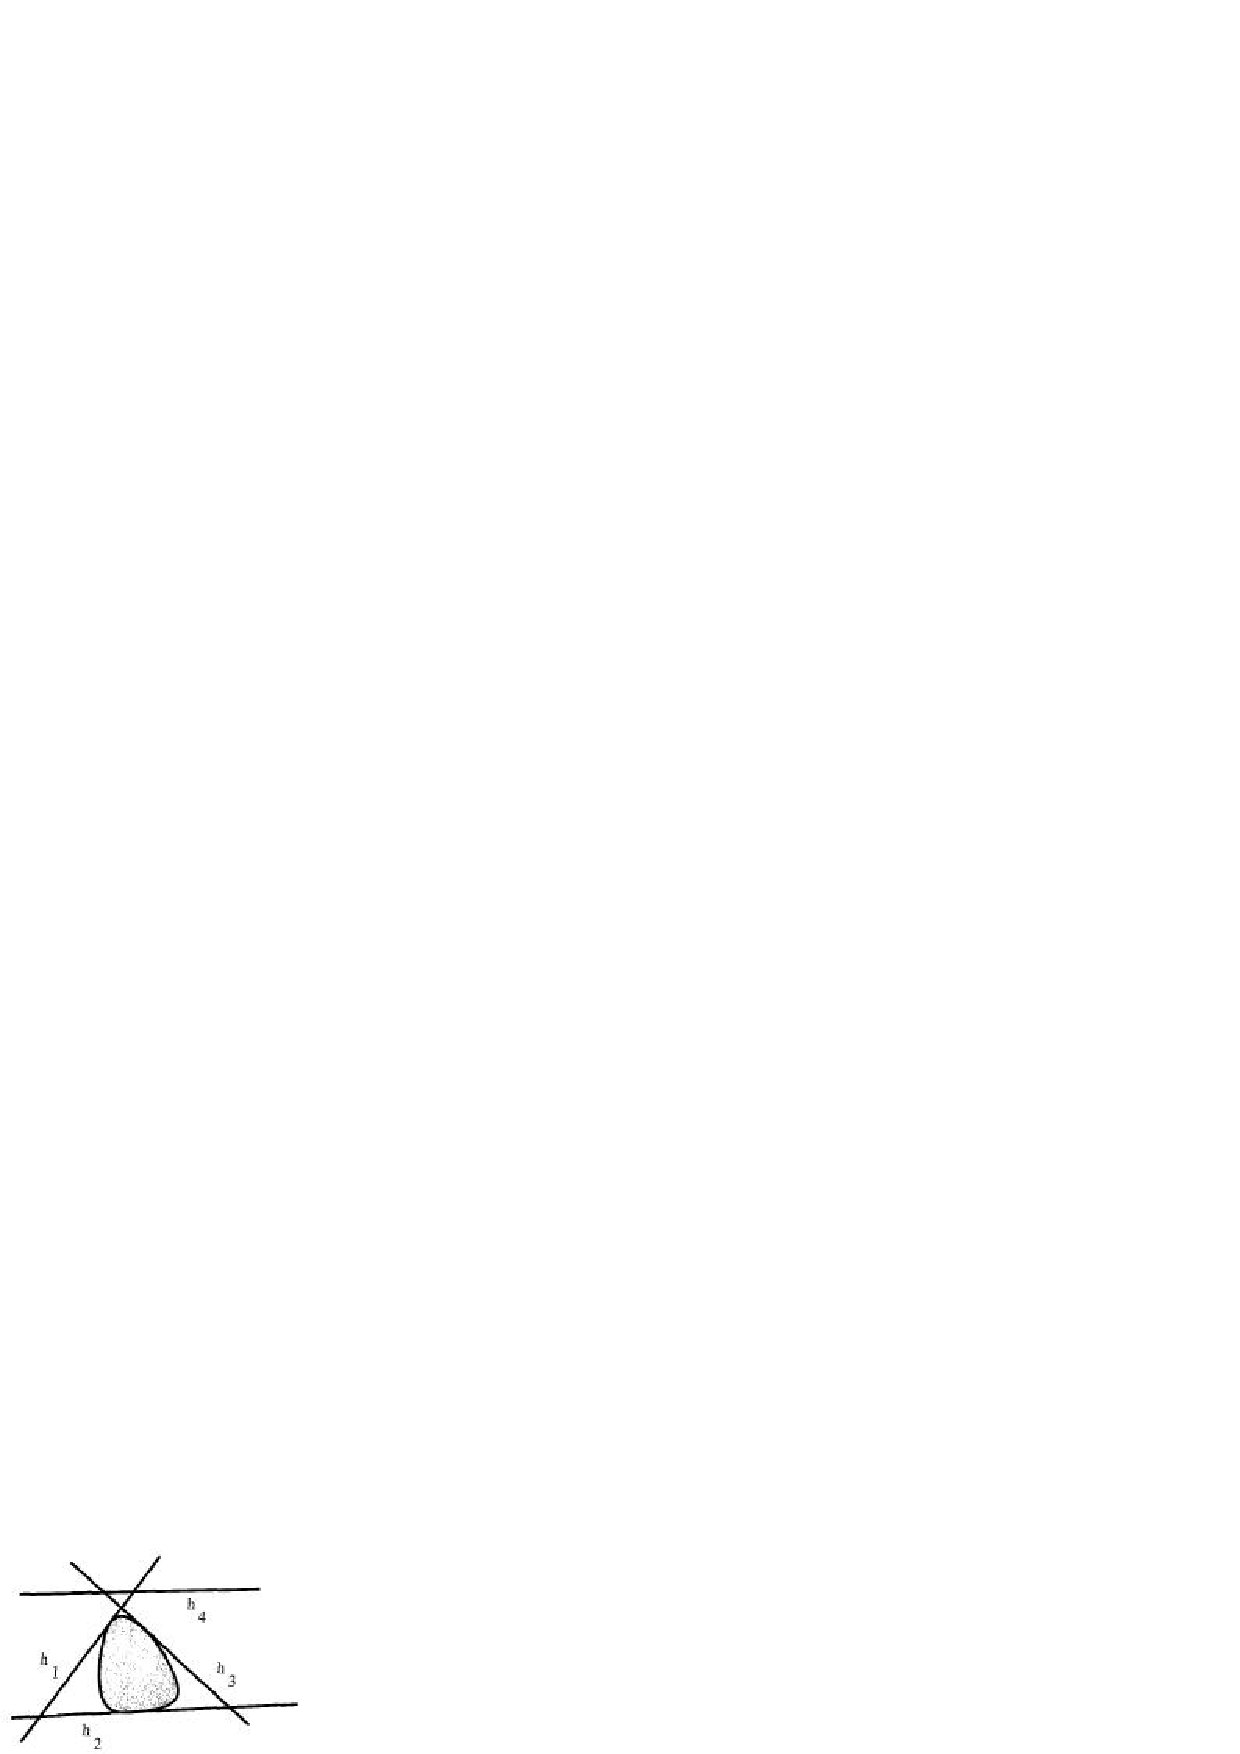
\includegraphics{images/inconsistent-support-planes.jpg}
 \end{center}
 \caption{Пример несогласованных опорных чисел}
 \label{image:inconsistent}
\end{wrapfigure}

Оказывается, не всякий набор вещественных чисел является набором согласованных
опорных чисел (см. рис. \ref{image:inconsistent}).

Чтобы показать, насколько это важно, определим (следуя
\cite{Prince:1990:RCS:81024.81035}) так называемый \textit{основной объект} ---
тело, которое можно восстановить из опорных чисел, если о нем неизвестны никакие
другие априорные данные:

\begin{SmartDefinition}
 \label{def:basic-object}
 \textbf{Основным объектом} опорных чисел $h_{1}, h_{2}, \ldots, h_{m}$ по
 направлениям $u_{1}, u_{2}, \ldots, u_{m}$ называется многогранник $K^{0}$,
 определяемый как пересечение полупространств, ограниченных опорными плоскостями
 и содержащими начало координат $O$:
 \begin{equation}
  K^{0} = \bigcap \limits_{i = 1}^{m}\{(x, u_{i}) \leq h_{i}\}
 \end{equation}
\end{SmartDefinition}

В случае, если одно из опорных чисел было получено с большой погрешностью, может
оказаться, что заметная часть опорных чисел не будут учтена при построении
основного объекта. Так возникает вопрос \textit{построения оценки опорной
функции} --- такого набора согласованных опорных чисел
$h^{*} = (h^{*}_{1}, h^{*}_{2}, \ldots, h^{*}_{m})$, который был бы в некотором
смысле ближайшим к набору исходных чисел
$h^{0} = (h^{0}_{1}, h^{0}_{2}, \ldots, h^{0}_{m})$
, т. е. являлся бы решением следующей задачи
минимизации:

\begin{equation}
 \label{equation:abstract-problem}
 ||h - h^{0} ||_{X} \to \inf, \;\;\;\; s. t. \;\; h \in \mathfrak{C}
\end{equation}

где $X$ --- некоторая метрика в $\mathbb{R}^{n}$, а
$\mathfrak{C} \subset \mathbb{R}^{m}$ --- множество всех согласованных наборов
опорных чисел по направлениям $u_{1}, u_{2}, \ldots, u_{m}$.

\textbf{3. Исторический обзор.} Описанный выше подход для двумерного случая был
разработан в статьях Prince и Willsky \cite{Prince:1990:RCS:81024.81035},
изучавшими данные из компьютерной томографии,  и Lele, Kulkarni и Willsky
\cite{Lele:92}, изучавшими данные, полученные из лазерного радара. В них
доказывается так называемая \textbf{опорная теорема}:

\begin{SmartTheorem}
 \label{theorem:support-theorem}
  Набор опорных чисел $h = (h_{1}, h_{2}, \ldots, h_{m})$ по направлениям
  $u_{i} = (\cos \theta_{i}, \sin \theta_{i}) \in \mathbb{R}^{2},
  i = 1, \ldots, m$ является согласованным тогда и только тогда, когда

  \begin{equation}
   C h \geq 0
  \end{equation}

  где $C$ --- так называемая \textbf{опорная матрица}:
 \begin{equation}
  \left(
  \begin{array}{ccccccc}

   \scriptstyle     -sin(\theta_{2} - \theta_{M}) &
   \scriptstyle     sin(\theta_{1} - \theta_{M}) &
   \scriptstyle     0 &
   \scriptstyle     \ldots &
   \scriptstyle     0 &
   \scriptstyle     0 &
   \scriptstyle     sin(\theta_{2} - \theta_{1}) \\

   \scriptstyle      sin(\theta_{3} - \theta_{2}) &
   \scriptstyle      -sin(\theta_{3} - \theta_{1}) &
   \scriptstyle      sin(\theta_{2} - \theta_{1}) &
   \scriptstyle      \ldots &
   \scriptstyle      0 &
   \scriptstyle      0 &
   \scriptstyle      0 \\

   \scriptstyle      0 &
   \scriptstyle      sin(\theta_{4} - \theta_{3}) &
   \scriptstyle      -sin(\theta_{4} - \theta_{2}) &
   \scriptstyle      \ldots &
   \scriptstyle      0 &
   \scriptstyle      0 &
   \scriptstyle      0 \\

   \scriptstyle      \vdots &
   \scriptstyle      \vdots &
   \scriptstyle      \vdots &
   \scriptstyle      \ddots &
   \scriptstyle      \vdots &
   \scriptstyle      \vdots &
   \scriptstyle      \vdots \\

   \scriptstyle      0 &
   \scriptstyle      0 &
   \scriptstyle      0 &
   \scriptstyle      \ldots &
   \scriptstyle      -sin(\theta_{m - 1} - \theta_{m - 3}) &
   \scriptstyle      sin(\theta_{m - 2} - \theta_{m - 3}) &
   \scriptstyle      0 \\

   \scriptstyle      0 &
   \scriptstyle      0 &
   \scriptstyle      0 &
   \scriptstyle      \ldots &
   \scriptstyle      sin(\theta_{m} - \theta_{m - 1}) &
   \scriptstyle      -sin(\theta_{m} - \theta_{m - 2}) &
   \scriptstyle      sin(\theta_{m - 1} - \theta_{m - 2}) \\

   \scriptstyle      sin(\theta_{m} - \theta_{m - 1}) &
   \scriptstyle      0 &
   \scriptstyle      0 &
   \scriptstyle      \ldots &
   \scriptstyle      0 &
   \scriptstyle      sin(\theta_{1} - \theta_{m}) &
   \scriptstyle      -sin(\theta_{1} - \theta_{m - 1}) \\
  \end{array}
  \right)
 \end{equation}

\end{SmartTheorem}

Таким образом, множество всех согласованных наборов опорных чисел представляет
из себя конус, называемый \textit{опорным конусом}:

\begin{equation}
 \mathfrak{C} = \{h \in \mathbb{R}^{m} \; | \; C h \geq 0\}
\end{equation}

Следовательно, задача минимизации (\ref{equation:abstract-problem}) является
задачей квадратичного программирования в метрике $L_{2}$ и задачей линейного
программирования в метрике $L_{1}$:

\begin{equation}
 \label{equation:general-problem}
 ||h - h^{0} ||_{X} \to \inf, \;\;\;\; s. t. \;\; C h \geq 0
\end{equation}

Авторы приводят результаты решения этих задач минимизации, проводят анализ их
быстродействия, а также предлагают подходы, позволяющие учитывать априорные
знания о восстанавливаемых телах (такие как, например, кривизна).

Более сложным является рассмотрение задачи в трехмерном случае. Аналог теоремы
\ref{theorem:support-theorem} для трехмерного случая был доказан Karl, Kulkarni,
Verghese и Willsky \cite{Karl:1996:LTC:234032.234054}.

\begin{SmartTheorem}
 Набор опорных чисел $h = (h_{1}, h_{2}, \ldots, h_{m})$ по направлениям
 $u_{1}, u_{2}, \ldots, u_{m} \in \mathbb{R}^{3}$ является согласованным тогда и
 только тогда, когда неравенство

 \begin{equation}
 \label{equation:consistency-3d}
\left|\begin{array}{cc}
  h_{i} & u_{i}^{T} \\
  h_{j} & u_{j}^{T} \\
  h_{k} & u_{k}^{T} \\
  h_{l} & u_{l}^{T} \\
\end{array}\right|
  \left|\begin{array}{cc}
  1 & u_{i}^{T} \\
  1 & u_{j}^{T} \\
  1 & u_{k}^{T} \\
  1 & u_{l}^{T} \\
\end{array}\right|
\geq 0
\end{equation}

выполнено для всех четвёрок индексов $\{i, j, k, l\}$ таких, что сферический
треугольник, образованный векторами $u_{i}, u_{j}, u_{k}$ содержит в своей
внутренности вектор $u_{l}$ и не содержит никаких других опорных направлений из
$u_{1}, \ldots, u_{m}$ (такие четвёрки называются локальными положительными
конусами).
\end{SmartTheorem}

Таким образом, в трехмерном случае множество $\mathfrak{C}$ всех согласованных
опорных числе представляет из себя опорный конус, задаваемый уравнением
$C h \geq 0$, в котором строки опорной матрицы $C$ составлены из коэффициентов
уравнения (\ref{equation:consistency-3d}).

Авторы не доказали в статье оценок о количестве условий вида
(\ref{equation:consistency-3d}), однако произвели численный эксперимент по
построению условий для случайно выбранных опорных направлений. Из его
результатов можно предположить, что для случайно выбранных направлений число
уравнений растет примерно как $O(m^{2})$ (возможно, с логарифмическим
множителем).

Данный алгоритм был реализован Gregor и Rannou для данных из \\
магнитно-резонансной визуализации в статьях \cite{IMA:IMA10007} и
\cite{doi:10.1117/12.431168}. При этом авторы столкнулись с тем, что при больших
размерностях (порядка 100000 опорных направлений) время поиска локальных
положительных четвёрок было на порядок больше, чем время решения самой задачи
квадратичного программирования.

В связи с этим Gardner и Kiderlen \cite{4586384} решили переформулировать
исходную задачу в терминах точек касания:

\begin{equation}
\label{equation:gardner-kiderlen}
 ||\{(x_{i}, u_{i})\}_{i = 1}^{m} - h^{0}|| \to \inf \;\;\; s. t. \;\;
 (x_{i}, u_{i}) \geq (x_{j}, u_{i}), 1 \leq i \neq j \leq m
\end{equation}

где $x_{i} \in \mathbb{R}^{3}$ --- точки касания тела с опорной плоскостью,
имеющей нормаль $u_{i}$. Как нетрудно видеть, если решить задачу оптимизации
(\ref{equation:gardner-kiderlen}), то по полученным точкам касания $x^{*}_{i}$
можно получить согласованные опорные числа $h^{*}_{i} = (x^{*}_{i}, u_{i})$, а
по ним --- восстановить основной объект.

Преимущество данного подхода состоит в том, что условия согласованности
выписываются автоматически, и для их нахождения не требуется искать все
локальные положительные конусы. Тем не менее, основная проблема данного подхода,
а именно квадратичное число условий, сохраняется в данной постановке задачи.

\bibliographystyle{plain}
\bibliography{307167,81035,josaa-9-10-1693,234054,10.10022Fima.10007,906585citation,4586384}

\end{document}
